% Seeded from ../notebooks/lesson_37.ipynb; source notebook is unchanged.
% Reading and focus: ../pages/lesson_37.md (assigned reading and macro objective).
% Cell indices in provenance comments are zero-based, matching the ipynb array.
% Markdown, Python, and meaningful stored outputs are retained; no notebook execution is required.
\documentclass[compact]{ne630handout}
\handoutsolutionsfalse
\begin{document}
% Notebook cell 0 (markdown)
\Lesson{37}{The Reflected Reactor}{Lewis, Sec.~7.5.}{Students will be able to characterize both quantitatively and qualitatively the impact of a reflector region on an otherwise bare reactor core using diffusion theory.}
\begin{handoutflow}

\textbf{LAST TIME}: The two-group criticality problem.

\textbf{TODAY}: The reflected reactor.

\textbf{NEXT TIME}: Modeling reactor control (and control ``worth'').
% End notebook cell 0

% Notebook cell 1 (markdown)
\Sec{1}{Review: The Bare Slab Reactor}

Consider a slab reactor of width \(a\), for which the one-group diffusion equation is

\[
   \frac{d^2 \phi}{dx^2} + \overbrace{\frac{k_{\infty}/k-1}{L^2}}^{B^2} = 0
    \quad \longrightarrow \quad \phi(x) = C_1 \cos(Bx) \, .
\]
% End notebook cell 1

% Notebook cell 2 (markdown)
For zero-flux conditions, we have

\[
  B^2 = \left ( \frac{\pi}{a} \right )^2
\]
% End notebook cell 2

% Notebook cell 3 (markdown)
For extrapolated-flux conditions (with \(\lambda = 1/\Sigma_{tr} = 3D\)), we have

\[
   B^2 = \left ( \frac{\pi/2}{\frac{a}{2}+\frac{2\lambda}{3}} \right )^2 = \left ( \frac{\pi}{a+4D} \right )^2
\]
% End notebook cell 3

% Notebook cell 4 (markdown)
For vacuum conditions, we found the transcendental equation

\[
 \boxed{ \cot{\frac{Ba}{2}} = 2BD } \, .
 \tag{criticality condition}
\]
% End notebook cell 4

% Notebook cell 5 (markdown)
Given \(B^2\), it we have

\[
   k = \frac{k_{\infty}}{1+L^2 B^2} \, .
\]
% End notebook cell 5

% Notebook cell 6 (code)
\begin{NEunicodecode}
import numpy as np
D = 1.0; Σ_a = 0.1; a = 50;  L = np.sqrt(D/Σ_a); λ = 3*D;  k_oo = 1.3;
\end{NEunicodecode}
% End notebook cell 6

% Notebook cell 7 (code)
\begin{NEunicodecode}
B_squared = (np.pi/a)**2;   k = k_oo / (1+L**2*B_squared);
print(f"B^2 = {B_squared:.5f}   k = {k:.5f}")
\end{NEunicodecode}
% Stored notebook output 0 (text/plain).
\begin{NEunicodecode}
B^2 = 0.00395   k = 1.25063
\end{NEunicodecode}
% End notebook cell 7

% Notebook cell 8 (code)
\begin{NEunicodecode}
B_squared = (np.pi/(a+4*D))**2;   k = k_oo / (1+L**2*B_squared);
print(f"B^2 = {B_squared:.6f}   k = {k:.5f}")
\end{NEunicodecode}
% Stored notebook output 0 (text/plain).
\begin{NEunicodecode}
B^2 = 0.003385   k = 1.25744
\end{NEunicodecode}
% End notebook cell 8

% Notebook cell 9 (code)
\begin{NEunicodecode}
cot = lambda x: np.cos(x)/np.sin(x)
f = lambda B: cot(B*a/2)-2*B*D
from scipy.optimize import fsolve
B = fsolve(f, np.pi/a)[0]
B_squared = B**2;   k = k_oo / (1+L**2*B_squared);
print(f"B^2 = {B_squared:.6f}   k = {k:.5f}")
\end{NEunicodecode}
% Stored notebook output 0 (text/plain).
\begin{NEunicodecode}
B^2 = 0.003387   k = 1.25741
\end{NEunicodecode}
% End notebook cell 9

% Notebook cell 10 (markdown)
In other words, the extrapolated flux condition is only \emph{approximating} the vacuum condition!
% End notebook cell 10

% Notebook cell 11 (markdown)
\Sec{2}{The Reflected Reactor}
% End notebook cell 11

% Notebook cell 12 (markdown)
The idea is simple: replace the vacuum with something that causes neutrons to scatter back into the reactor.
% End notebook cell 12

% Notebook cell 13 (markdown)
A good reflector has a \textbf{small \(\Sigma_a\)} and \textbf{large \(\Sigma_s\)}.
% End notebook cell 13

% Notebook cell 14 (markdown)
\begin{center}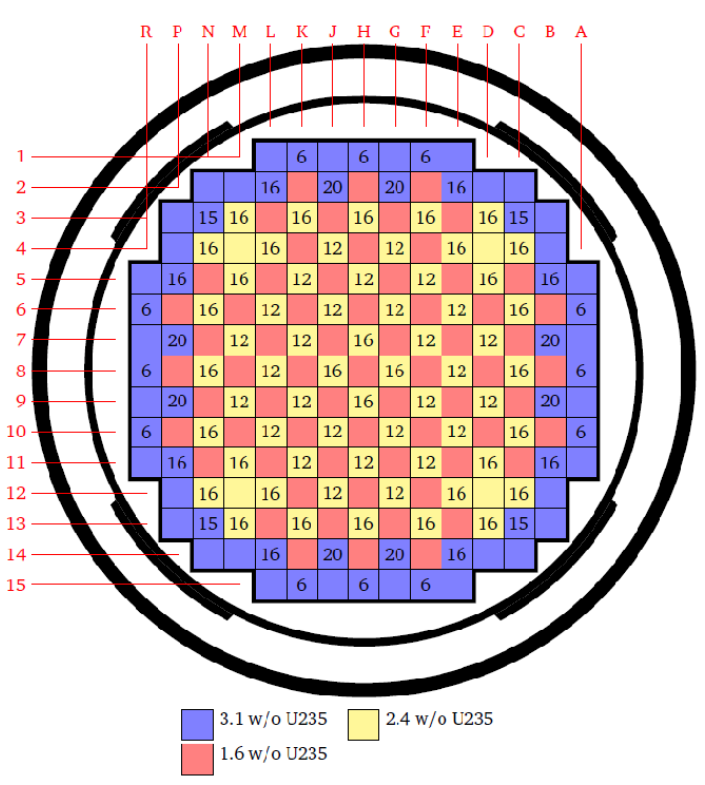
\includegraphics[width=\linewidth,height=.37\textheight,keepaspectratio]{figures/notebook_37/cell_14_attachment.png}\end{center}

{[}Diagram from the MIT BEAVRS Benchmark Specification (based on a commercial PWR){]}
% End notebook cell 14

% Notebook cell 15 (markdown)
\begin{center}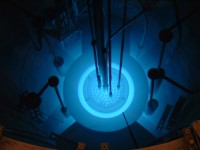
\includegraphics[width=\linewidth,height=.37\textheight,keepaspectratio]{figures/notebook_37/cell_15_attachment.png}\end{center}

{[}K-State TRIGA{]}
% End notebook cell 15

% Notebook cell 16 (markdown)
\Sec{3}{Example: The Reflected Slab}
% End notebook cell 16

% Notebook cell 17 (markdown)
In the fuel region (call that region I), nothing changes:

\[
  \phi_{I}(x) = C_1 \cos(Bx) \, .
\]
% End notebook cell 17

% Notebook cell 18 (markdown)
\Needspace{6\baselineskip}
In the reflector region, there is no fission, so \(-\phi_{II}'' + (1/L^2)\phi_{II}(x) = 0\) and

\[
 \phi_{II}(x) = C_2 \cosh(x/L) + C_3 \sinh(x/L) \, .
\]
% End notebook cell 18

% Notebook cell 19 (code)
\begin{NEunicodecode}
import sympy as sy
D_I, D_II, Sigma_a, a, t, B, L = sy.symbols("D_I, D_II, Sigma_a, a, t, B, L_II", positive=True)
C1, C2, C3 = sy.symbols("C1, C2, C3")
x = sy.symbols("x", real=True)
phi_I = C1*sy.cos(B*x)
phi_II = C2*sy.cosh(x/L) + C3*sy.sinh(x/L)
\end{NEunicodecode}
% End notebook cell 19

% Notebook cell 20 (markdown)
First, we apply the outer boundary condition (assuming vacuum) so that

\[
  \frac{\phi_{II}(a/2+t)}{4} + \frac{D_{II}}{2} \frac{d\phi_{II}}{dx} \Big |_{x=a/2+t} = 0 \, .
\]
% End notebook cell 20

% Notebook cell 21 (code)
\begin{NEunicodecode}
bc = sy.Eq( phi_II.subs(x, a/2+t)/4 + (D_II/2)*sy.diff(phi_II, x).subs(x, a/2+t), 0)
bc
\end{NEunicodecode}
% Stored notebook output 0 (text/latex).
\[
\displaystyle \frac{C_{2} \cosh{\left(\frac{\frac{a}{2} + t}{L_{II}} \right)}}{4} + \frac{C_{3} \sinh{\left(\frac{\frac{a}{2} + t}{L_{II}} \right)}}{4} + \frac{D_{II} \left(\frac{C_{2} \sinh{\left(\frac{\frac{a}{2} + t}{L_{II}} \right)}}{L_{II}} + \frac{C_{3} \cosh{\left(\frac{\frac{a}{2} + t}{L_{II}} \right)}}{L_{II}}\right)}{2} = 0
\]
% End notebook cell 21

% Notebook cell 22 (markdown)
Then, we can eliminate one of the coefficients:
% End notebook cell 22

% Notebook cell 23 (code)
\begin{NEunicodecode}
coefs = sy.solve([bc], C2)
\end{NEunicodecode}
% End notebook cell 23

% Notebook cell 24 (code)
\begin{NEunicodecode}
coefs[C2].simplify()
\end{NEunicodecode}
% Stored notebook output 0 (text/latex).
\[
\displaystyle - \frac{C_{3} \cdot \left(2 D_{II} \cosh{\left(\frac{\frac{a}{2} + t}{L_{II}} \right)} + L_{II} \sinh{\left(\frac{\frac{a}{2} + t}{L_{II}} \right)}\right)}{2 D_{II} \sinh{\left(\frac{\frac{a}{2} + t}{L_{II}} \right)} + L_{II} \cosh{\left(\frac{\frac{a}{2} + t}{L_{II}} \right)}}
\]
% End notebook cell 24

% Notebook cell 25 (markdown)
Now, our reflector flux depends only on \(C_3\):
% End notebook cell 25

% Notebook cell 26 (code)
\begin{NEunicodecode}
phi_II_sol = phi_II.subs(coefs).simplify()
phi_II_sol
\end{NEunicodecode}
% Stored notebook output 0 (text/latex).
\[
\displaystyle - \frac{C_{3} \cdot \left(2 D_{II} \cosh{\left(\frac{\frac{a}{2} + t - x}{L_{II}} \right)} + L_{II} \sinh{\left(\frac{\frac{a}{2} + t - x}{L_{II}} \right)}\right)}{2 D_{II} \sinh{\left(\frac{\frac{a}{2} + t}{L_{II}} \right)} + L_{II} \cosh{\left(\frac{\frac{a}{2} + t}{L_{II}} \right)}}
\]
% End notebook cell 26

% Notebook cell 27 (markdown)
Remember, \textbf{SymPy is being used here only for algebra}!
% End notebook cell 27

% Notebook cell 28 (markdown)
Now, the continuity conditions:

\[
   \phi_I(a/2) = \phi_{II}(a/2)
   \tag{flux continuity}
\]

and

\[
  -D_I\phi_I'(a/2) = -D_{II} \phi_{II}'(a/2) \, .
  \tag{current continuity}
\]
% End notebook cell 28

% Notebook cell 29 (markdown)
The trick: note that both fluxes have an arbitrary constant (\(C_1\) and \(C_3\)). So, we can divide the current continuity equation by the flux continuity equation to get a new criticality condition:
% End notebook cell 29

% Notebook cell 30 (code)
\begin{NEunicodecode}
LHS = (sy.diff(D_I*phi_I, x)/phi_I).subs(x, a/2).simplify()
LHS
\end{NEunicodecode}
% Stored notebook output 0 (text/latex).
\[
\displaystyle - B D_{I} \tan{\left(\frac{B a}{2} \right)}
\]
% End notebook cell 30

% Notebook cell 31 (code)
\begin{NEunicodecode}
RHS = (sy.diff(D_II*phi_II_sol, x)/phi_II_sol).subs(x, a/2).simplify()
\end{NEunicodecode}
% End notebook cell 31

% Notebook cell 32 (code)
\Needspace{8\baselineskip}
\begin{NEunicodecode}
criticality_condition = sy.Eq(LHS, RHS)
criticality_condition
\end{NEunicodecode}
% Stored notebook output 0 (text/latex).
\[
\displaystyle - B D_{I} \tan{\left(\frac{B a}{2} \right)} = - \frac{D_{II} \left(2 D_{II} \sinh{\left(\frac{t}{L_{II}} \right)} + L_{II} \cosh{\left(\frac{t}{L_{II}} \right)}\right)}{L_{II} \left(2 D_{II} \cosh{\left(\frac{t}{L_{II}} \right)} + L_{II} \sinh{\left(\frac{t}{L_{II}} \right)}\right)}
\]
% End notebook cell 32

% Notebook cell 33 (markdown)
In the limit that the reflector is infinitely thick, we have
% End notebook cell 33

% Notebook cell 34 (code)
\begin{NEunicodecode}
criticality_condition = sy.Eq(LHS, sy.limit(RHS, t, sy.oo))
criticality_condition
\end{NEunicodecode}
% Stored notebook output 0 (text/latex).
\[
\displaystyle - B D_{I} \tan{\left(\frac{B a}{2} \right)} = - \frac{D_{II}}{L_{II}}
\]
% End notebook cell 34

% Notebook cell 35 (markdown)
This is equivalent to Eq. (7.69) in the text (with \(\alpha^2 = 1/L_{II}^2\)). Solving for \(a\) yields
% End notebook cell 35

% Notebook cell 36 (code)
\begin{NEunicodecode}
sy.Eq(a, sy.solve(criticality_condition, a)[0])
\end{NEunicodecode}
% Stored notebook output 0 (text/latex).
\[
\displaystyle a = \frac{2 \operatorname{atan}{\left(\frac{D_{II}}{B D_{I} L_{II}} \right)}}{B}
\]
% End notebook cell 36

% Notebook cell 37 (markdown)
\Sec{4}{Example}

Suppose our two-region data is as entered below (where the region I data is the same as our initial bare reactor material). How wide must the reflected reactor be to have the same multiplication as the bare core assuming an infinitely thick reflector?
% End notebook cell 37

% Notebook cell 38 (code)
\begin{NEunicodecode}
import numpy as np
D_I = 1.0; Σ_a_I = 0.1; a = 50;  L_I = np.sqrt(D_I/Σ_a_I); k_oo = 1.3;
D_II = 0.9; Σ_a_II = 0.01; L_II = np.sqrt(D_II/Σ_a_II);
B_bare = np.sqrt(0.003387)
\end{NEunicodecode}
% End notebook cell 38

% Notebook cell 39 (code)
\begin{NEunicodecode}
a_prime = np.arctan(D_II/(B_bare*D_I*L_II))/B_bare
print(f"a' = {a_prime:.4f} cm")
\end{NEunicodecode}
% Stored notebook output 0 (text/plain).
\begin{NEunicodecode}
a' = 17.5356 cm
\end{NEunicodecode}
% End notebook cell 39

% Notebook cell 40 (markdown)
\Sec{5}{Summary}

For our \textbf{bare} reactor, we needed to satisfy the criticality condition

\[
  \cot{\frac{Ba}{2}} = 2BD_I  \, .
\]

and for \(D_I = 1\) cm, \(\Sigma_a = 0.1\) 1/cm, \(k_{\infty} = 1.3\), and \(a = 50\) cm, we found

\[
B^2 = 0.003387 \qquad \text{and} \qquad  k = 1.25741 \, .
\]
% End notebook cell 40

% Notebook cell 41 (markdown)
For the \textbf{reflected} reactor (with an \emph{infinitely thick reflector}), the modified criticality condition is

\[
  a' = \frac{2 \operatorname{atan}{\left(\frac{D_{II}}{B D_{I} L_{II}} \right)}}{B}
\]

where \(a'\) is the width of the reflected reactor, and for the same values
% End notebook cell 41

% Notebook cell 42 (markdown)
The key point: \(a' = 17.5356\) cm is \emph{much less than} \(a = 50\) cm for the same value of \(B^2\) (and, hence, \(k\)).
% End notebook cell 42

% Notebook cell 43 (markdown)
The book defines the \textbf{reflector savings} specifically as \(\delta_x = (1/2)(a-a')\), so our savings would be
% End notebook cell 43

% Notebook cell 44 (code)
\begin{NEunicodecode}
print(f"reflector savings = {0.5*(a-a_prime):.4f} cm")
\end{NEunicodecode}
% Stored notebook output 0 (text/plain).
\begin{NEunicodecode}
reflector savings = 16.2322 cm
\end{NEunicodecode}
% End notebook cell 44

\end{handoutflow}
\end{document}
